%storm
\documentclass[../../main/main.tex]{subfiles}


\begin{document}
\title{Background}


%%%%%%%%%%%%%%%%%%%%% Chapter STORM %%%%%%%%%%%%%%%
\chapter{STORM}\label{chp:srorm}

%%%%%%%%%%%%%%%%%%%%% Section SE %%%%%%%%%%%%%%%
\section{Systems Engineering}\label{sec:stormse}
"Systems Engineering is an interdisciplinary approach and means to enable the realization of successful systems. It focuses on defining customer needs and required functionality early in the development cycle, documenting requirements, then proceeding with design synthesis and system validation while considering the complete problem: Operations, Performance, Test, Manufacturing, Cost \& Schedule, Training \& Support, Disposal."

International Council on Systems Engineering 

A system is a set of interacting and interdependent components that act as a whole,  through various mechanisms, to perform some function. Systems engineering is a multidisciplinary approach to solving problems related to large and complex man-made systems.  It focuses on stakeholder needs and assets while minimizing asset losses.  It focuses on building the right product.  It avoids building the wrong product or building the right product incorrectly.  

According to Holstein and Bode's, who summarized systems engineering for the Encyclopedia Britannica, systems engineering probably developed from the overlapping of engineering concepts from different fields. They note that, for example, both chemical and mechanical engineering focus on heat transfer, and cybernetics and computer theory are both subdisciplines of electrical and electronics engineering.   But, at its core is the scientific methodology and the use of mathematical modeling.  Holstein and Bode link the more recent emergence of systems engineering to the communications industry (telephony, in particular) and Britain's post-World War II operations research.

The emergence of systems engineering and its growing popularity is linked to the growing complexity of systems.  Systems are composed more and more of numerous interacting parts.  These interacting parts often exhibit emergent properties.  These are properties that arise from the interactions of many components.  These properties are not attributable to any one component and thus require a systems-thinking perspective. Holstein and Bode site the Nike Ajax U.S. Air Defense System as one of the earlier examples of these system-level emergent properties. Tactical range of the Ajax requires consideration of multiple factors including aerodynamic design, maneuverability provided by the control systems, warhead size and weight, etc.  Other factors include feedback from radar and the autopilot.

Systems engineering is often employed in the communications and computing industries. But, it works in any field that works with large complex systems.  The applicability of systems engineering to other fields is promoted, in part, by the increased capacity to manage complex systems that arise from the increased computational power available.  Systems engineering is a growing field and demands for systems engineers will continue to grow as systems become more and more complex.

Authoritative guidelines and standards on systems engineering can be found in ISO/IEC/IEEE 24748-1 and ISO/IEC/IEEE 25288.  These works describe six distinct phases of a system's life cycle: concept, development, production, utilization, support, and retirement.  Typically, the STROM methodology demonstrated in this master thesis focuses on the concept and development phase systems engineering. This is because it is intended to be used to inform a safe and secure system design.  However, for this particular master thesis, this work could be viewed as a support phase activity. This is because the system to which we are applying STORM has already been designed and employed in the field.   Support, in this aspect, entails re-envisioning the system from a safety and security perspective with the use of more modern tools that tackle the problems that arise from complexity.
%%%%%%%%%%%%%%%%%%%%% Section SSE %%%%%%%%%%%%%%%
\section{Systems Security Engineering}\label{sesc:sse}
"The ultimate objective is to obtain trustworthy secure systems that are fully capable of supporting critical missions and business operations while protecting stakeholder assets, and to do so with a level of assurance that is consistent with the risk tolerance of those stakeholders."
Ron Ross (NIST) (Quoted from NIST SP 800-160)

Systems Security Engineering \glsentryshort{sse} is a subdiscipline of Systems Engineering.  It applies scientific, mathematical, and related technical concepts and procedures to engineer trustworthy systems that meet stakeholder needs. 

Systems Security Engineering probably developed alongside systems engineering.  But, the need for security in all systems is becoming more and more evident in today's technology-dependent society.  In the authoritative document on SSE (National institute for Standardization and Technology (NIST) Special Publication 800-160 vol 1), the abstract states

"With the continuing frequency, intensity, and adverse consequences of cyber-attacks, disruptions, hazards, and other threats to federal, state, and local governments, the military, businesses, and the critical infrastructure, the need for trustworthy secure systems has never been more important to the long-term economic and national security interests of the United States. Engineering-based solutions are essential to managing the growing complexity, dynamicity, and interconnectedness of today?s systems, as exemplified by cyber-physical systems and systems-of-systems, including the Internet of Things."

Systems Security Engineering is practiced whenever security is a component of systems engineering.  As a subspecialty of systems engineering, SSE focuses on stakeholder assets and loss avoidance or mitigation.  It is a multidisciplinary approach that considers emergent properties which arise from the complexity of large systems.
   

\subsection{Systems Security Engineering Framework}
The authoritative document on SSE is the National Institute of Standardization and Technology (NIST) Special Publication 800-160 Volumes 1 and 2.  In particular, volume 1 defines the SSE Framework.  This framework defines SSE activities that ensure the stakeholder's definition of security and asset valuation is understood.  A diagram of the framework is shown in figure \ref{sseframework}.

\begin{figure}[h]
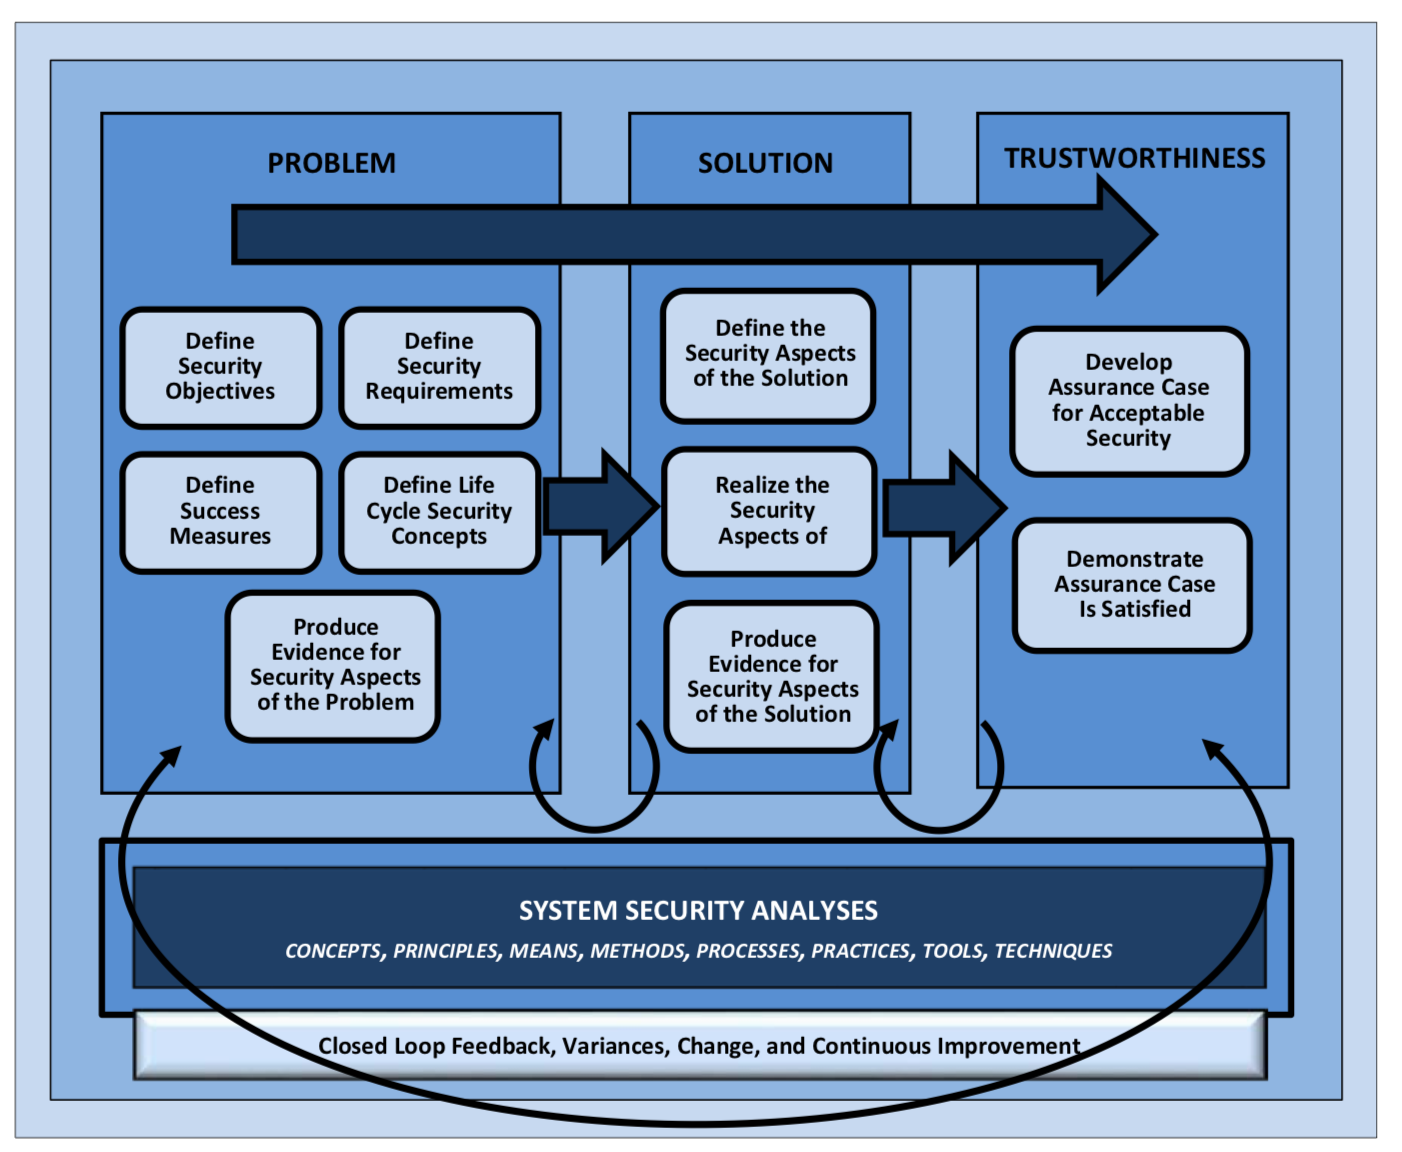
\includegraphics[width=\linewidth]{../figures/sseframework}
\caption{\label{sseframework}Systems security engineering Framework. (Image from \glsentryshort{nist} Special Publication 800-160 Vol 1: Systems Security Engineering Considerations for a Multidisciplinary Approach in the Engineering of Trustworthy Secure Systems.)}
\end{figure}

\paragraph*{Problem}
The framework describes the problem, solution, and trustworthiness activity contexts.  These three contexts are further broken down.  The problem phase focuses on defining security from the stakeholder's needs, purpose, and mission.  It is divided into four subcategories.  The first category defines the security objective. What does it means to be "\textit{adequately secure}"?   What are the assets and asset losses?  Which losses are unacceptable?
 
The second category in the problem context is to define measures of success.  What level of asset protection is required?  What level of assurance or protection is required?  

The third subcategory is to define the system life-cycle security concepts.  What is the system security context throughout the life-cycle of the system?  What processes, methods, and procedures throughout the system's life cycle need security?  

The fourth subcategory is to define the security requirements.  The stakeholder security requirements are determined from the previous three subcategories.

\paragraph*{Solution}
With the problem defined, the solution activity transforms the problem into security design requirements.  This a three part process.  The first subcategory in the solution context is to define the security aspects of the solution. NIST SP 800-160 lists six aspects to focus on: protection strategy; security design requirements; security architecture view and viewpoints; security design; security procedural aspects, capabilities, and limitations in the system life-cycle; and how to verify and measure security performance. 

The next subcategory is to realize the security aspects.  This is the security implementation phase.

The last subcategory in the solution context is to produce evidence for the security aspects of the solution. This assurance evidence can be obtained from a variety of SSE verification methods.  Assurance claims are measured against the stakeholder's requirements.

\paragraph*{Trustworthiness}
Once the solution is generated, the trustworthiness context provides evidence that the system is trustworthy.  The evidence supports the security objective claims.  There are two subcategories of activities in this context.  The first is to develop and maintain that assurance case for acceptable security.  NIST SP 800-160 defines assurance case as \textit{"a well-defined and structured set of arguments and a body of evidence showing that a system satisfies specific claims with respect to a given quality attribute."}  Assurance cases also provide auditable artifacts supporting the system security claims.

The other trustworthiness activity is to demonstrate that the assurance case is satisfied.  As subject-matter expert should evaluate the assurance case to determine if the evidence supports the security claims.

\subsubsection{Conforming to The SSE Framework}
STORM conforms to the SSE Framework.  The two components of STORM (described next) are STPA and CSBD.  STPA focuses on the problem and solution contexts of the framework.  The problem is defined in step 1 of STPA.  The solutions is defined in steps 2, 3, and 4. CSBD focuses on demonstrating trustworthiness through formal methods and computer-aided reasoning.  It uses a rigorous mathematical logic to verify claims of security with regards to confidentiality, integrity, and accessibility.  

The work in this master thesis applies the STORM methodology to patrol base operations.  Therefore, this work also conforms to the SSE Framework.


%%%%%%%%%%%%%%%%%%%%% Section STORM %%%%%%%%%%%%%%%
\section{STORM}\label{sec:storm}

%%%%%%%%%%%%%%%%%%%%% Subsection STORM %%%%%%%%%%%%%%%
\subsection{STAMP}\label{ssec:stamp}

%%%%%%%%%%%%%%%%%%%%% Subsection STORM %%%%%%%%%%%%%%%
\subsection{STPA \& STPA-Sec}\label{ssec:stpa}

%%%%%%%%%%%%%%%%%%%%% Subsection STORM %%%%%%%%%%%%%%%
\subsubsection{XSTAMPP}\label{sssec:xstamp}


%%%%%%%%%%%%%%%%%%%%% Subsection STORM %%%%%%%%%%%%%%%
\subsection{CSBD}\label{ssec:csbd}


%%%%%%%%%%%%%%%%%%%%% Subsection STORM %%%%%%%%%%%%%%%
\subsubsection{Confidentiality, Integrity, and Accessibility (CIA) }\label{sssect:ssmts}


%%%%%%%%%%%%%%%%%%%%% Subsection STORM %%%%%%%%%%%%%%%
\subsubsection{Complete Mediation}\label{sssec:strommediate}

%%%%%%%%%%%%%%%%%%%%% Subsection STORM %%%%%%%%%%%%%%%
\subsubsection{Secure State Machines as Transition Systems }\label{sssect:ssmts}

%%%%%%%%%%%%%%%%%%%%% Section PB %%%%%%%%%%%%%%%
\section{Patrol Base Operations}\label{sec:stormpb}

\end{document}